% Phase 1 Presentation: EM + Chemistry Coupling in TEL ICP Etcher
% Compile: pdflatex slides.tex
\documentclass[aspectratio=169,10pt]{beamer}

\usetheme{default}
\usecolortheme{default}
\setbeamertemplate{navigation symbols}{}
\setbeamertemplate{footline}[frame number]
\setbeamertemplate{frametitle}{\vskip0.2cm\insertframetitle}

\usepackage{amsmath,amssymb}
\usepackage{booktabs}
\usepackage{graphicx}
\usepackage{siunitx}
\usepackage{xcolor}
\usepackage{tikz}
\usetikzlibrary{arrows.meta, positioning}

\graphicspath{{../report/figures/}}

% Custom macros
\newcommand{\SFsix}{\mathrm{SF}_6}
\newcommand{\SFfive}{\mathrm{SF}_5}
\newcommand{\Te}{T_e}
\newcommand{\eV}{\,\mathrm{eV}}

\title{Digital Twin Plasma Model:\\
  EM Field Computation and Self-Consistent Coupling\\
  with SF$_6$/Ar Chemistry in an ICP Etcher}
\author{Muhammad Abdelghany \and Zachariah Ngan}
\institute{Illinois Plasma Institute\\
  University of Illinois at Urbana-Champaign}
\date{April 2026}


\begin{document}

% ══════════════════════════════════════════
\begin{frame}
  \titlepage
\end{frame}

% ══════════════════════════════════════════
\begin{frame}{Outline}
  \tableofcontents
\end{frame}


% ══════════════════════════════════════════════════════════════
\section{Motivation \& Architecture}
% ══════════════════════════════════════════════════════════════

% ──────────────────────────────────────────
\begin{frame}{ICP Etchers in Semiconductor Fabrication}
  \begin{columns}[T]
    \begin{column}{0.55\textwidth}
      \begin{itemize}[]
        \item Inductively Coupled Plasma (ICP) reactors dominate anisotropic etching below \SI{10}{\nano\meter} nodes
        \item TEL ICP etcher: 6-inch wafer, HF \SI{40}{\mega\hertz} \SI{700}{\watt}
        \item Key challenge: predict \textbf{etch uniformity} from first-principles physics
        \item Mettler (2025) measured 74\% centre-to-edge [F] drop via radical probes
        \item \textbf{Goal}: replace prescribed plasma parameters with self-consistent EM + chemistry coupling
      \end{itemize}
    \end{column}
    \begin{column}{0.42\textwidth}
      \centering
      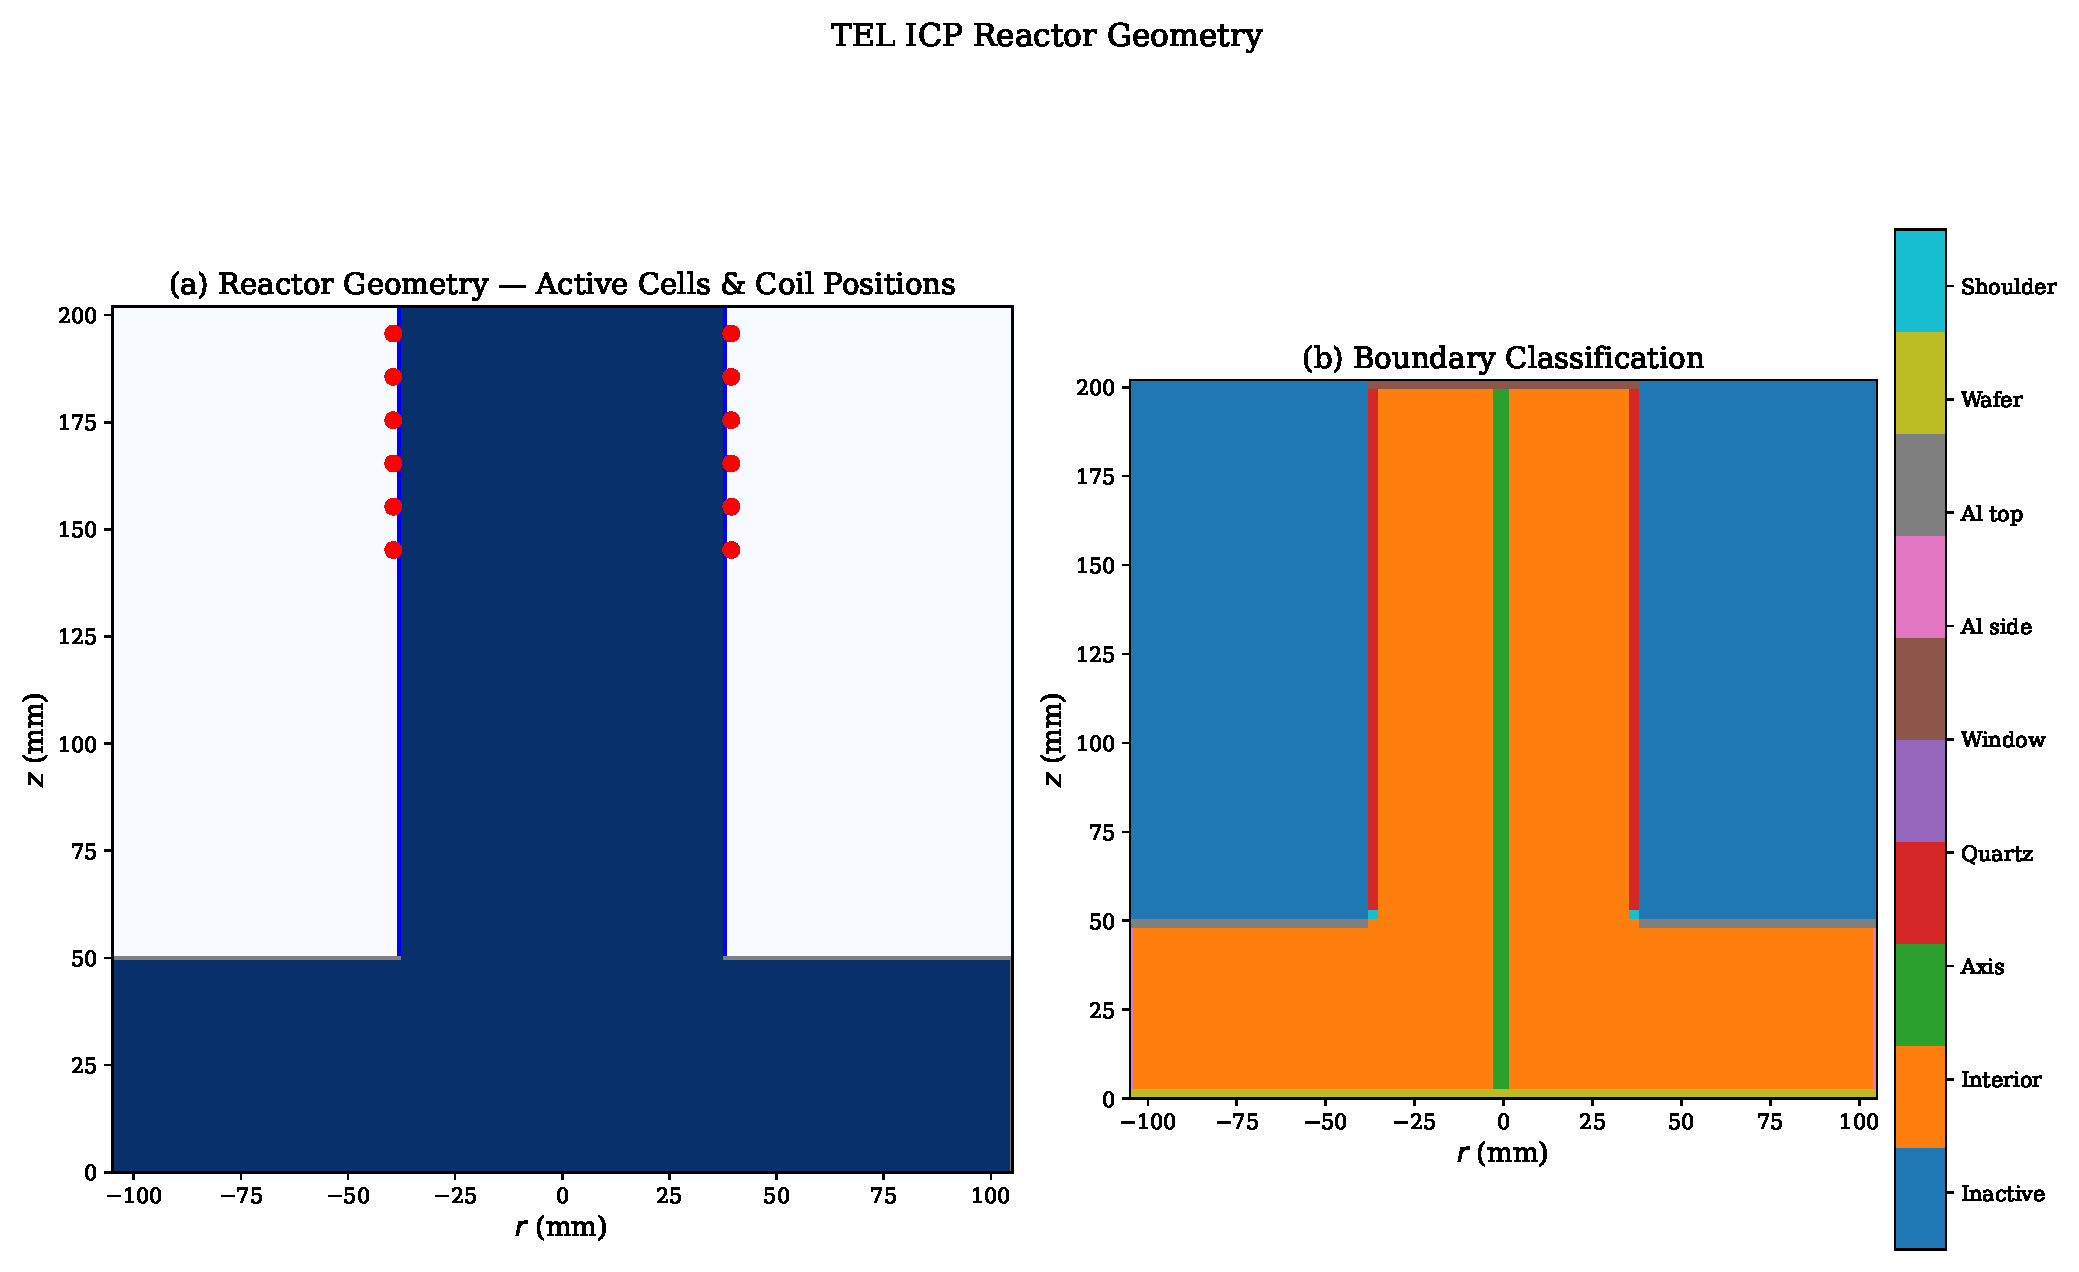
\includegraphics[width=\textwidth,height=0.65\textheight,keepaspectratio]{fig01_geometry}
    \end{column}
  \end{columns}
\end{frame}

% ──────────────────────────────────────────
\begin{frame}{DTPM Pipeline Architecture}
  \begin{center}
    \footnotesize
    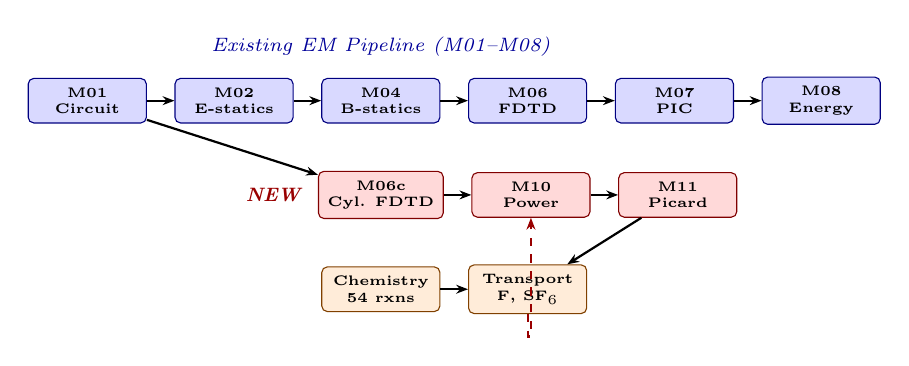
\begin{tikzpicture}[node distance=0.35cm,
      modbox/.style={rectangle, draw, rounded corners=2pt, minimum width=1.5cm, minimum height=0.55cm, align=center, font=\tiny\bfseries},
      embox/.style={modbox, fill=blue!15, draw=blue!50!black},
      newbox/.style={modbox, fill=red!15, draw=red!50!black},
      chembox/.style={modbox, fill=orange!15, draw=orange!50!black},
      arr/.style={-{Stealth[length=1.5mm]}, thick}]
      \node[embox] (m01) {M01\\Circuit};
      \node[embox, right=of m01] (m02) {M02\\E-statics};
      \node[embox, right=of m02] (m04) {M04\\B-statics};
      \node[embox, right=of m04] (m06) {M06\\FDTD};
      \node[embox, right=of m06] (m07) {M07\\PIC};
      \node[embox, right=of m07] (m08) {M08\\Energy};
      \node[newbox, below=0.6cm of m04] (m06c) {M06c\\Cyl. FDTD};
      \node[newbox, right=of m06c] (m10) {M10\\Power};
      \node[newbox, right=of m10] (m11) {M11\\Picard};
      \node[chembox, below=0.6cm of m06c] (chem) {Chemistry\\54 rxns};
      \node[chembox, right=of chem] (trans) {Transport\\F, SF$_6$};
      \draw[arr] (m01) -- (m02); \draw[arr] (m02) -- (m04);
      \draw[arr] (m04) -- (m06); \draw[arr] (m06) -- (m07);
      \draw[arr] (m07) -- (m08);
      \draw[arr] (m01) -- (m06c); \draw[arr] (m06c) -- (m10);
      \draw[arr] (m10) -- (m11);
      \draw[arr] (chem) -- (trans); \draw[arr] (m11) -- (trans);
      \draw[arr, dashed, red!60!black] (trans) -- ++(0,-0.6) -| (m10);
      \node[above=0.15cm of m04, font=\scriptsize\itshape, blue!60!black] {Existing EM Pipeline (M01--M08)};
      \node[left=0.1cm of m06c, font=\scriptsize\itshape, red!60!black] {\textbf{NEW}};
    \end{tikzpicture}
  \end{center}
  \vspace{0.2cm}
  \begin{itemize}[]
    \item Each module: \texttt{run(state, config) -> dict} --- merged into shared state
    \item \textcolor{red!60!black}{\textbf{Phase 1 additions}}: M06c (cylindrical FDTD), M10 (power deposition), M11 (Picard coupling)
    \item Picard loop: EM $\to$ power $\to$ $T_e$ $\to$ $n_e$ $\to$ chemistry $\to$ repeat
  \end{itemize}
\end{frame}


% ══════════════════════════════════════════════════════════════
\section{Part I: Electromagnetic Pipeline}
% ══════════════════════════════════════════════════════════════

% ──────────────────────────────────────────
\begin{frame}{M01: RF Circuit Analysis}
  \begin{columns}[T]
    \begin{column}{0.55\textwidth}
      For matched RF source with power $P$ into impedance $Z$:
      \begin{align}
        V_\text{rms} &= \sqrt{P\,Z} \\
        V_\text{peak} &= V_\text{rms}\sqrt{2} \\
        I_\text{peak} &= \frac{V_\text{rms}}{Z}\sqrt{2} \\
        \omega &= 2\pi f
      \end{align}
    \end{column}
    \begin{column}{0.42\textwidth}
      \centering
      \footnotesize
      \begin{tabular}{@{}ll@{}}
        \toprule
        Parameter & Value \\
        \midrule
        $P$ & \SI{700}{\watt} \\
        $f$ & \SI{40}{\mega\hertz} \\
        $Z$ & \SI{50}{\ohm} \\
        \midrule
        $V_\text{peak}$ & \SI{264.6}{\volt} \\
        $I_\text{peak}$ & \SI{5.29}{\ampere} \\
        $\omega$ & \SI{2.51e8}{\radian/\second} \\
        \bottomrule
      \end{tabular}
    \end{column}
  \end{columns}
\end{frame}

% ──────────────────────────────────────────
\begin{frame}{M02: Electrostatic Field Solver}
  \begin{columns}[T]
    \begin{column}{0.5\textwidth}
      Laplace equation in the reactor:
      \[
        \nabla^2 \Phi = 0
      \]
      Solved via Gauss--Seidel SOR with Red-Black ordering:
      \[
        \Phi_{i,j}^{n+1} = (1{-}\omega)\Phi_{i,j}^n + \frac{\omega}{4}
        \!\left(\Phi_{i\pm1,j}^{*} + \Phi_{i,j\pm1}^{*}\right)
      \]
      Electric field from central differences:
      \[
        E_x = -\frac{\partial\Phi}{\partial x},\quad
        E_y = -\frac{\partial\Phi}{\partial y}
      \]
    \end{column}
    \begin{column}{0.47\textwidth}
      \begin{itemize}[]
        \item Dirichlet BC: $\Phi = V_\text{peak}$ at coils, $\Phi = 0$ at walls
        \item Relaxation $\omega = 1.8$
        \item Convergence: $\max|\Delta\Phi| < 10^{-2}$
        \item Red-Black ordering enables vectorisation
      \end{itemize}
    \end{column}
  \end{columns}
\end{frame}

% ──────────────────────────────────────────
\begin{frame}{M04: Magnetostatic Field (Elliptic Integrals)}
  Exact axisymmetric solution for circular coil at $(a, z_c)$:
  \[
    k^2 = \frac{4\,a\,r}{(a+r)^2 + (z-z_c)^2}
  \]
  \begin{align}
    B_z &= \frac{\mu_0 I}{2\pi}\frac{1}{\sqrt{(a{+}r)^2{+}(z{-}z_c)^2}}
    \left[K(k) + \frac{a^2{-}r^2{-}(z{-}z_c)^2}{(a{-}r)^2{+}(z{-}z_c)^2}E(k)\right] \\
    B_r &= \frac{\mu_0 I}{2\pi r}\frac{z{-}z_c}{\sqrt{(a{+}r)^2{+}(z{-}z_c)^2}}
    \left[-K(k) + \frac{a^2{+}r^2{+}(z{-}z_c)^2}{(a{-}r)^2{+}(z{-}z_c)^2}E(k)\right]
  \end{align}
  \begin{itemize}[]
    \item $K(k)$, $E(k)$: complete elliptic integrals of 1st and 2nd kind
    \item Superposition from $N$ coil turns; no segmentation error
  \end{itemize}
\end{frame}

% ──────────────────────────────────────────
\begin{frame}{M05--M06: FDTD Electromagnetic Wave Simulation}
  \begin{columns}[T]
    \begin{column}{0.48\textwidth}
      Maxwell's equations (TM mode):
      \begin{align}
        \frac{\partial H_x}{\partial t} &= -\frac{1}{\mu_0}\frac{\partial E_z}{\partial y} \\[4pt]
        \frac{\partial H_y}{\partial t} &= +\frac{1}{\mu_0}\frac{\partial E_z}{\partial x} \\[4pt]
        \frac{\partial E_z}{\partial t} &= \frac{1}{\epsilon_0}\!\left(\frac{\partial H_y}{\partial x} - \frac{\partial H_x}{\partial y}\right)
      \end{align}
      \vspace{0.1cm}
      Mur 1st-order ABC:
      \[
        E_z^{n+1}[0] = E_z^n[1] + \frac{c\Delta t - \Delta x}{c\Delta t + \Delta x}\!\left(E_z^{n+1}[1] - E_z^n[0]\right)
      \]
    \end{column}
    \begin{column}{0.48\textwidth}
      \begin{itemize}[]
        \item Yee-grid staggering: $E_z$ at cell centers, $H_x$, $H_y$ at faces
        \item Leapfrog: H at $t+\frac{1}{2}\Delta t$, E at $t+\Delta t$
        \item CFL: $\Delta t < \frac{\min(\Delta x,\Delta y)}{c\sqrt{2}}$
        \item Gaussian-modulated sinusoidal source
      \end{itemize}
    \end{column}
  \end{columns}
\end{frame}

% ──────────────────────────────────────────
\begin{frame}{M07: Particle-in-Cell (2D3V Boris Pusher)}
  \begin{columns}[T]
    \begin{column}{0.5\textwidth}
      \textbf{Boris leap-frog algorithm}:
      \begin{enumerate}[]
        \item Half electric kick: $\mathbf{v}^- = \mathbf{v}^n + \frac{q\Delta t}{2m}\mathbf{E}$
        \item B-rotation vectors:\\
          $\mathbf{t} = \frac{q\Delta t}{2m}\mathbf{B}$,\quad
          $\mathbf{s} = \frac{2\mathbf{t}}{1+|\mathbf{t}|^2}$
        \item Rotate: $\mathbf{v}' = \mathbf{v}^- + \mathbf{v}^-\!\times\!\mathbf{t}$\\
          $\mathbf{v}^+ = \mathbf{v}^- + \mathbf{v}'\!\times\!\mathbf{s}$
        \item Second half kick: $\mathbf{v}^{n+1} = \mathbf{v}^+ + \frac{q\Delta t}{2m}\mathbf{E}$
        \item Move: $\mathbf{x}^{n+1} = \mathbf{x}^n + \mathbf{v}^{n+1}\Delta t$
      \end{enumerate}
    \end{column}
    \begin{column}{0.47\textwidth}
      \begin{itemize}[]
        \item Cloud-in-Cell (CIC) bilinear weighting for charge deposit and field gather
        \item 5000 electron + 5000 ion macroparticles
        \item Maxwellian initialisation at $T_e = \SI{3}{\eV}$
        \item Energy conservation: $\sim 10^{-15}$ in pure B-field
      \end{itemize}
    \end{column}
  \end{columns}
\end{frame}


% ══════════════════════════════════════════════════════════════
\section{Part II: SF$_6$/Ar Plasma Chemistry}
% ══════════════════════════════════════════════════════════════

% ──────────────────────────────────────────
\begin{frame}{0D Global Model: Particle \& Power Balance}
  \begin{columns}[T]
    \begin{column}{0.5\textwidth}
      \textbf{Particle balance} ($\Te$ from Brentq):
      \[
        \nu_\text{iz}(\Te) + \frac{R_\text{Penn}}{n_e} = \nu_\text{att}(\Te) + k_w^+(1+\alpha)
      \]
      \textbf{Power balance} ($n_e$):
      \[
        P_\text{abs} = n_e \cdot R_\text{iz} \cdot \varepsilon_T \cdot e \cdot V
      \]
      Energy cost per ion-electron pair:
      \[
        \varepsilon_T = \varepsilon_c + \varepsilon_{iw} + 2\Te
      \]
    \end{column}
    \begin{column}{0.47\textwidth}
      \textbf{Electronegativity}:
      \[
        \alpha(1+\alpha) = \frac{R_\text{att}}{k_\text{rec}\,n_e}
      \]
      \vspace{0.2cm}
      \footnotesize
      \begin{tabular}{@{}ll@{}}
        \toprule
        Output & Value \\
        \midrule
        $\Te$ & \SI{2.3}{\eV} \\
        $n_e$ & \SI{9.0e17}{\per\meter\cubed} \\
        $\alpha$ & 1.5 \\
        \bottomrule
      \end{tabular}
    \end{column}
  \end{columns}
\end{frame}

% ──────────────────────────────────────────
\begin{frame}{54-Reaction SF$_6$/Ar Chemistry (Lallement 2009)}
  \footnotesize
  \begin{center}
    \begin{tabular}{@{}llc@{}}
      \toprule
      \textbf{Category} & \textbf{Example} & \textbf{Count} \\
      \midrule
      SF$_6$ dissociation & $\SFsix + e \to \SFfive + F + e$ & 5 \\
      SFx sequential & $\SFfive + e \to \mathrm{SF}_4 + F + e$ & 6 \\
      Dissociative ionization & $\SFsix + e \to \SFfive^+ + F + 2e$ & 12 \\
      Dissociative attachment & $\SFsix + e \to \SFsix^-$ & 7 \\
      Troe recombination & $\SFfive + F (+M) \to \SFsix$ & 6 \\
      Disproportionation & $\SFfive + \SFfive \to \mathrm{SF}_4 + \SFsix$ & 3 \\
      Ion-ion recombination & All $+$/$-$ pairs & 1 \\
      Ar reactions & $\mathrm{Ar} + e \to \mathrm{Ar}^+ + 2e$ & 5 \\
      Penning/quenching & $\mathrm{Ar}^* + \SFsix \to \SFfive^+ + F + e$ & 5 \\
      \midrule
      \textbf{Total} & & \textbf{50+} \\
      \bottomrule
    \end{tabular}
  \end{center}
  \vspace{0.2cm}
  \normalsize
  \textbf{Troe fall-off} (Ryan \& Plumb 1990): $k_\text{eff} = \dfrac{k_0[\mathrm{M}]}{1+P_r} \cdot F_c^{\left(1+[\log_{10} P_r]^2\right)^{-1}}$
\end{frame}

% ──────────────────────────────────────────
\begin{frame}{Wall Surface Chemistry (Kokkoris 2009)}
  \begin{columns}[T]
    \begin{column}{0.5\textwidth}
      \textbf{5-channel mechanism}:
      \begin{enumerate}[]
        \item F adsorption ($s_F$)
        \item SFx adsorption ($s_{\text{SFx}}$)
        \item Fluorination ($p_\text{fluor}$)
        \item Eley--Rideal ($p_\text{wr}$)
        \item F$_2$ recombination ($p_\text{FF}$)
      \end{enumerate}
      \vspace{0.2cm}
      Robin BC at wall:
      \[
        -D\frac{\partial n}{\partial \hat{n}} = \frac{\gamma\,v_\text{th}}{4}\,n
      \]
    \end{column}
    \begin{column}{0.47\textwidth}
      \centering
      \footnotesize
      \begin{tabular}{@{}lc@{}}
        \toprule
        Material & $\gamma_\text{Al}$ (F) \\
        \midrule
        Quartz (SiO$_2$) & 0.001 \\
        \textbf{Aluminium} & \textbf{0.18} \\
        Silicon (wafer) & 0.025 \\
        Window & 0.001 \\
        \bottomrule
      \end{tabular}
      \vspace{0.3cm}
      \normalsize
      $\gamma_\text{Al} = 0.18$ is the \textbf{single calibrated parameter}
      (to match Mettler 74\% [F] drop)
    \end{column}
  \end{columns}
\end{frame}

% ──────────────────────────────────────────
\begin{frame}{2D Species Transport on TEL Geometry}
  \begin{columns}[T]
    \begin{column}{0.5\textwidth}
      Diffusion-reaction PDE in cylindrical $(r,z)$:
      \[
        \frac{1}{r}\frac{\partial}{\partial r}\!\left(r\,D\frac{\partial n}{\partial r}\right)
        + \frac{\partial}{\partial z}\!\left(D\frac{\partial n}{\partial z}\right) + S - L\,n = 0
      \]
      \begin{itemize}[]
        \item L'H\^opital at axis: $\lim_{r\to0}\frac{1}{r}\frac{\partial}{\partial r}(r\frac{\partial n}{\partial r}) = 2\frac{\partial^2 n}{\partial r^2}$
        \item Sparse matrix (COO $\to$ CSR) + \texttt{spsolve}
        \item Under-relaxation: $n^{k+1} = (1{-}w)\,n^k + w\,n_\text{solve}$
      \end{itemize}
    \end{column}
    \begin{column}{0.47\textwidth}
      \centering
      \textbf{TEL Reactor}:\\[4pt]
      \footnotesize
      \begin{tabular}{@{}ll@{}}
        \toprule
        Parameter & Value \\
        \midrule
        $R_\text{icp}$ & \SI{38}{\milli\meter} \\
        $R_\text{proc}$ & \SI{105}{\milli\meter} \\
        $L_\text{icp}$ & \SI{181.5}{\milli\meter} \\
        $L_\text{proc}$ & \SI{50}{\milli\meter} \\
        Aperture & \SI{2}{\milli\meter} \\
        Grid & $50\times80$ \\
        Active cells & 1669 / 4000 \\
        \bottomrule
      \end{tabular}
    \end{column}
  \end{columns}
\end{frame}

% ──────────────────────────────────────────
\begin{frame}{Stage 10 Validation: 74\% [F] Drop}
  \begin{columns}[T]
    \begin{column}{0.5\textwidth}
      \begin{itemize}[]
        \item Mettler (2025): spatially resolved F radical probe in TEL ICP etcher
        \item Stage 10 model: prescribed $\eta = 0.43$, Bessel-cosine $n_e(r,z)$, scalar $\Te$
        \item \textbf{Result}: 74\% centre-to-edge [F] drop
        \item 1.3$\times$ absolute [F] overprediction (within calibration)
        \item Sensitivity: $\pm$10\% $\gamma_\text{Al}$ $\Rightarrow$ $\pm$5 pp [F] drop
      \end{itemize}
    \end{column}
    \begin{column}{0.47\textwidth}
      \centering
      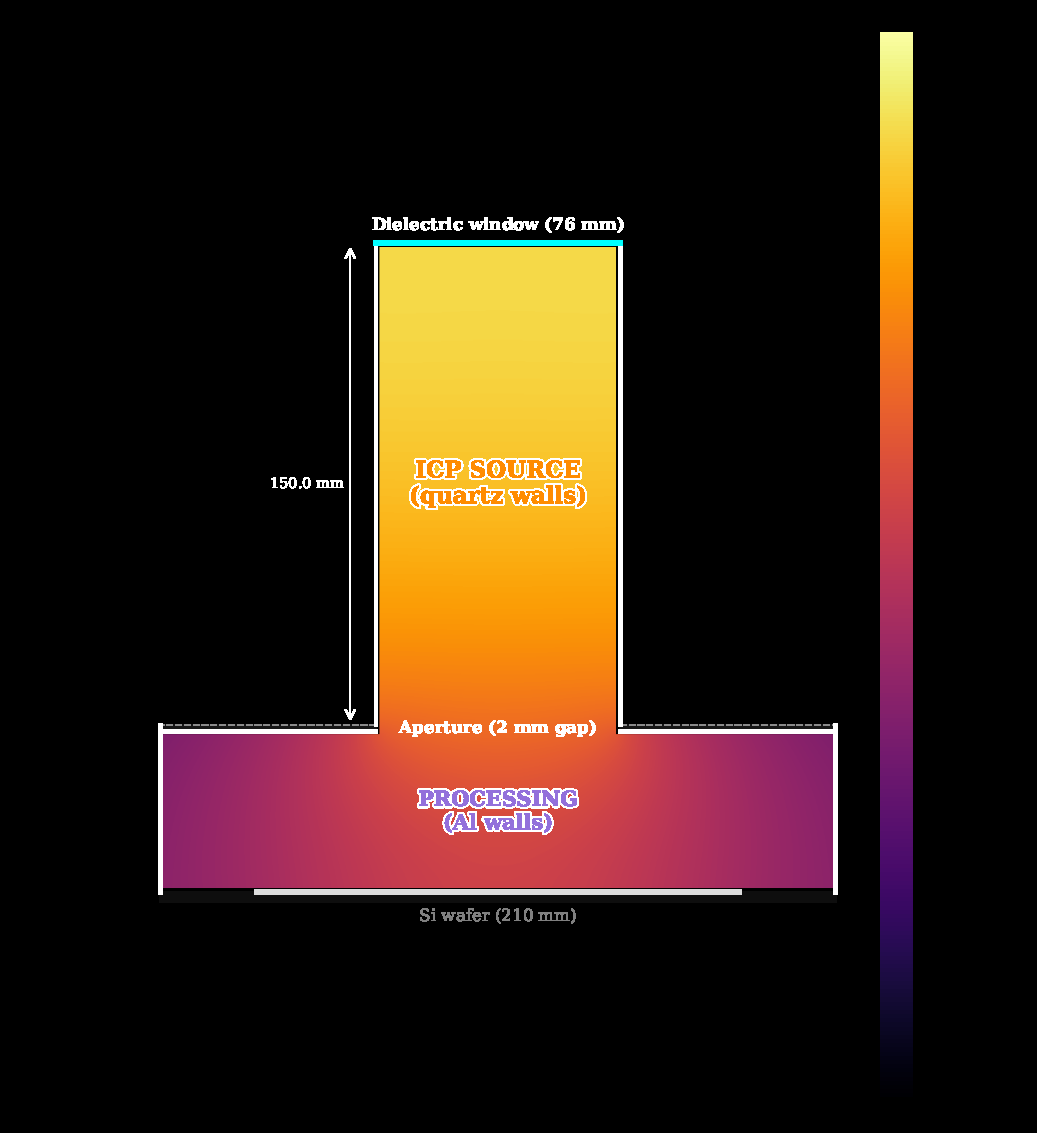
\includegraphics[width=\textwidth,height=0.65\textheight,keepaspectratio]{fig_cross_section_F}
    \end{column}
  \end{columns}
\end{frame}


% ══════════════════════════════════════════════════════════════
\section{Part III: Phase 1 --- EM + Chemistry Coupling}
% ══════════════════════════════════════════════════════════════

% ──────────────────────────────────────────
\begin{frame}{Cylindrical FDTD for ICP (M06c)}
  TE mode in axisymmetric $(r,z)$:
  \begin{align}
    \frac{\partial H_r}{\partial t} &= +\frac{1}{\mu_0}\frac{\partial E_\theta}{\partial z} \\
    \frac{\partial H_z}{\partial t} &= -\frac{1}{\mu_0}\frac{1}{r}\frac{\partial(r\,E_\theta)}{\partial r} \\
    \frac{\partial E_\theta}{\partial t} &= \frac{1}{\epsilon}\!\left(\frac{\partial H_r}{\partial z} - \frac{\partial H_z}{\partial r}\right) - \frac{\sigma}{\epsilon}E_\theta - \frac{J_\text{coil}}{\epsilon}
  \end{align}
  \begin{itemize}[]
    \item Source: $J_\theta = I_\text{peak}\sin(\omega t) / (\Delta r\,\Delta z)$ at coil positions
    \item Axis: $E_\theta(r{=}0) = 0$; L'H\^opital for $H_z$
    \item Quartz wall: $\epsilon_r = 3.8$ over \SI{3}{\milli\meter} thickness
    \item Vectorised numpy: \textbf{46$\times$ speedup} (30\,s on $50{\times}80$ grid)
  \end{itemize}
\end{frame}

% ──────────────────────────────────────────
\begin{frame}{FDTD Results: EM Fields at 40 MHz}
  \centering
  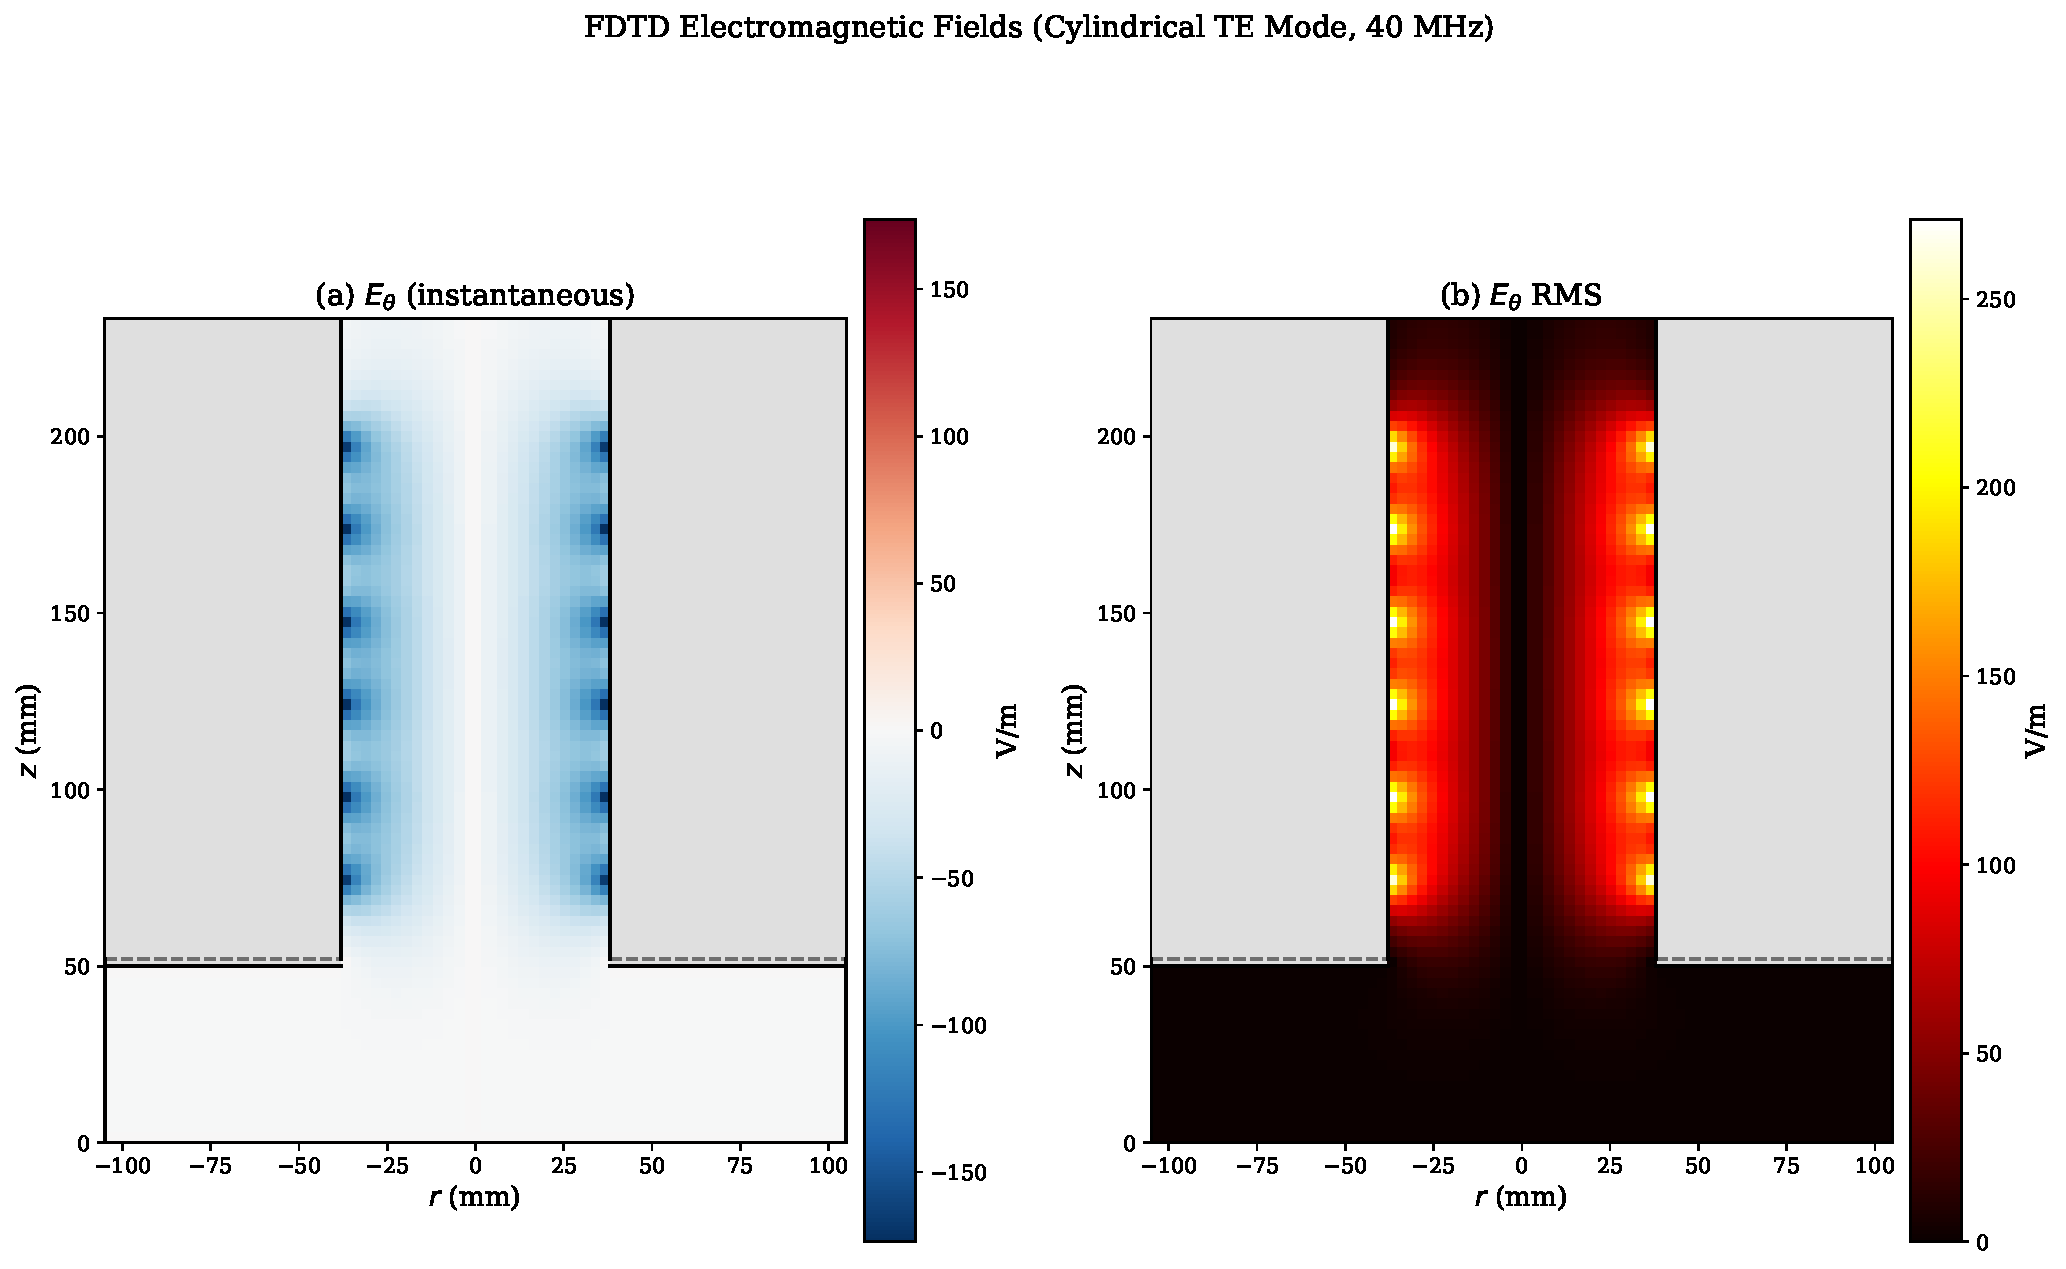
\includegraphics[width=0.95\textwidth,height=0.78\textheight,keepaspectratio]{fig_E_theta_fields}
  \vspace{0.1cm}

  \footnotesize
  $|E_{\theta,\text{rms}}|_\text{max} = \SI{456}{\volt/\meter}$ --- field peaks at skin depth near quartz wall
\end{frame}

% ──────────────────────────────────────────
\begin{frame}{Power Deposition (M10)}
  \begin{columns}[T]
    \begin{column}{0.5\textwidth}
      \[
        \boxed{P(r,z) = \frac{1}{2}\,\sigma(r,z)\,|E_{\theta,\text{rms}}|^2}
      \]
      Plasma conductivity:
      \[
        \sigma = \frac{e^2\,n_e}{m_e\,\nu_m},\quad \nu_m = n_g\,\langle\sigma_m v\rangle
      \]
      E-field normalisation:
      \[
        E_\text{scaled} = E_\text{FDTD}\cdot\sqrt{\frac{P_\text{target}}{P_\text{raw}}}
      \]
    \end{column}
    \begin{column}{0.47\textwidth}
      \centering
      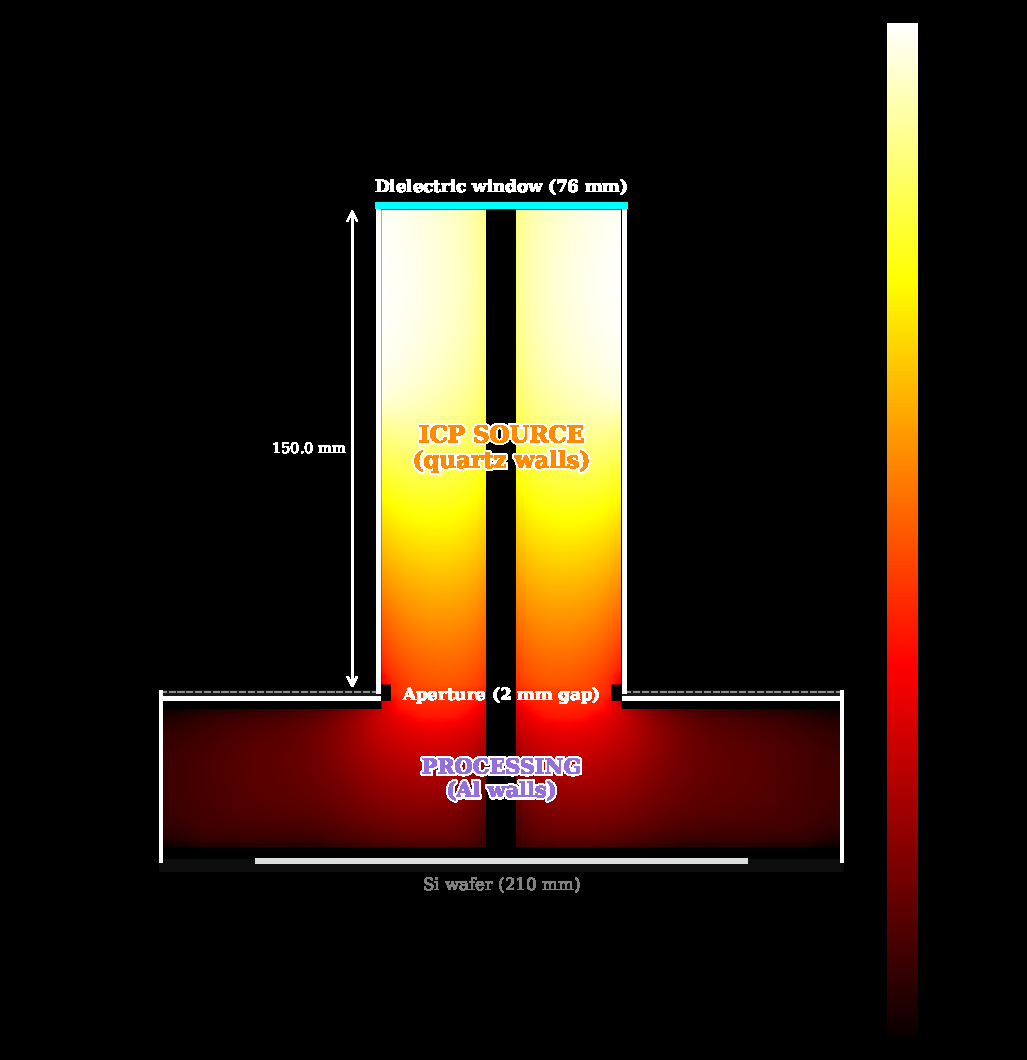
\includegraphics[width=\textwidth,height=0.6\textheight,keepaspectratio]{fig_power_deposition}
    \end{column}
  \end{columns}
\end{frame}

% ──────────────────────────────────────────
\begin{frame}{Ionization-Source Diffusion for $n_e(r,z)$}
  \begin{columns}[T]
    \begin{column}{0.52\textwidth}
      Steady-state electron continuity:
      \[
        \boxed{\nabla\!\cdot\!(D_a\nabla n_e) + S_\text{iz}(r,z) - \nu_\text{loss}\,n_e = 0}
      \]
      \begin{itemize}[]
        \item $S_\text{iz} = P(r,z)/(\varepsilon_T\,e)$ --- from FDTD power profile
        \item $D_a = D_i(1+\Te/T_i)$ --- ambipolar diffusion
        \item Robin BC: $D_a\,\partial n_e/\partial\hat{n} = -u_B\,n_e$
        \item Single sparse solve: $(A - \text{diag}(\nu_\text{loss}))\,n_e = -S_\text{iz}$
      \end{itemize}
      \vspace{0.2cm}
      \textbf{Key physics}: electrons born at skin depth (wall-peaked source) \textbf{diffuse inward} $\Rightarrow$ centre-peaked $n_e$
    \end{column}
    \begin{column}{0.45\textwidth}
      \centering
      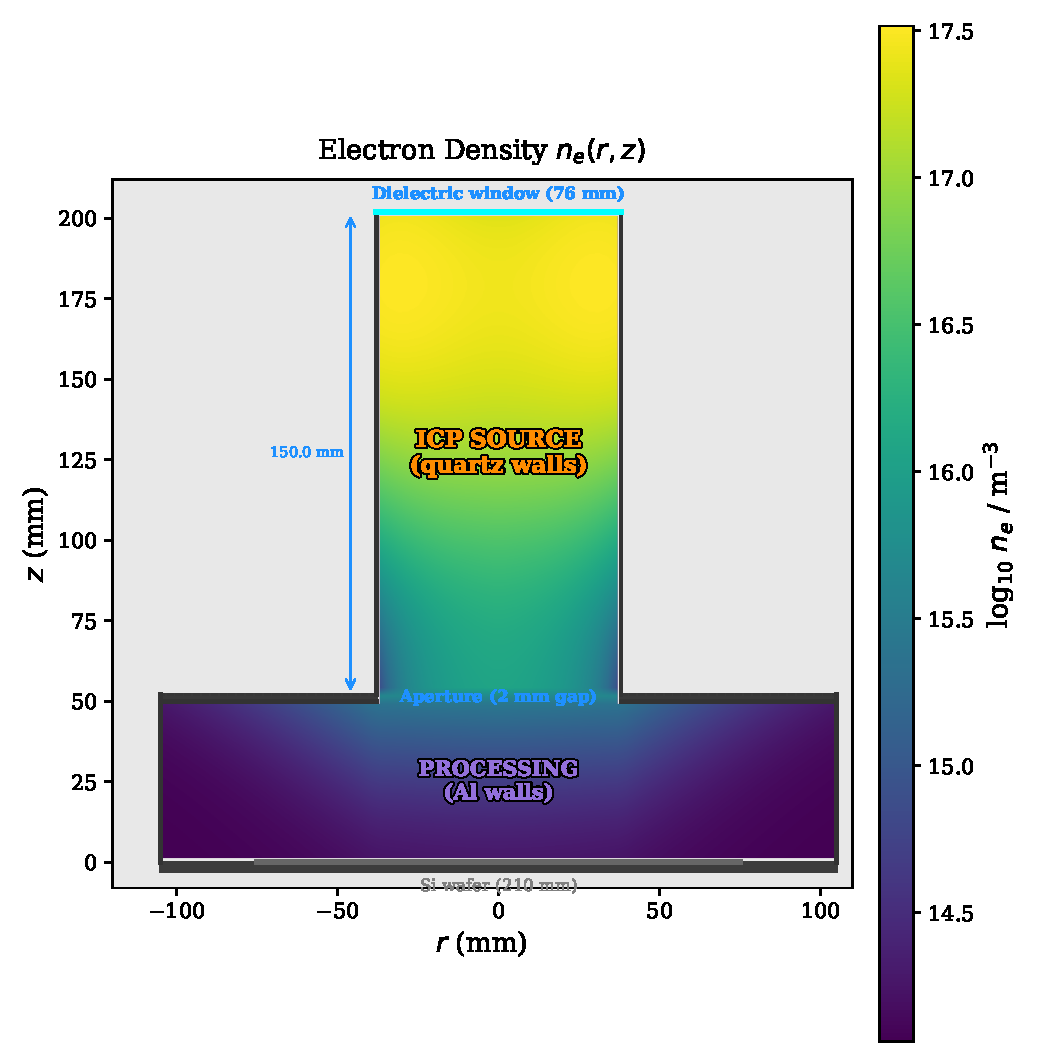
\includegraphics[width=\textwidth,height=0.65\textheight,keepaspectratio]{fig_ne_contour}
    \end{column}
  \end{columns}
\end{frame}

% ──────────────────────────────────────────
\begin{frame}{Picard Coupling Loop (M11)}
  \centering
  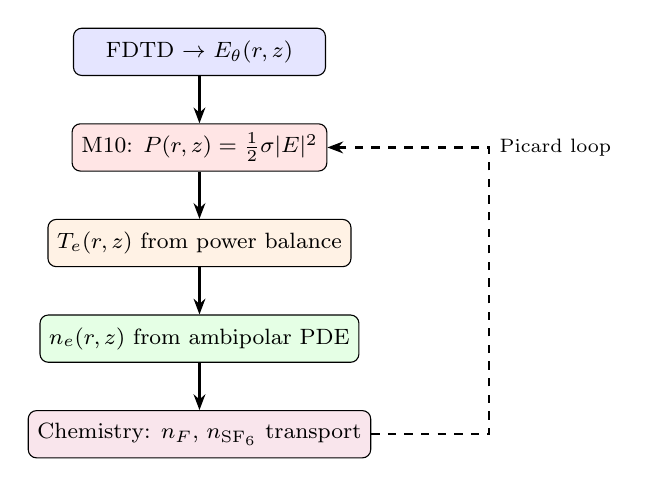
\begin{tikzpicture}[node distance=0.6cm,
    box/.style={rectangle, draw, rounded corners=3pt, minimum width=3.2cm, minimum height=0.6cm, font=\footnotesize, align=center},
    arr/.style={-{Stealth[length=2mm]}, thick}]
    \node[box, fill=blue!10] (fdtd) {FDTD $\to$ $E_\theta(r,z)$};
    \node[box, fill=red!10, below=of fdtd] (power) {M10: $P(r,z) = \frac{1}{2}\sigma|E|^2$};
    \node[box, fill=orange!10, below=of power] (Te) {$\Te(r,z)$ from power balance};
    \node[box, fill=green!10, below=of Te] (ne) {$n_e(r,z)$ from ambipolar PDE};
    \node[box, fill=purple!10, below=of ne] (chem) {Chemistry: $n_F$, $n_{\SFsix}$ transport};
    \draw[arr] (fdtd) -- (power);
    \draw[arr] (power) -- (Te);
    \draw[arr] (Te) -- (ne);
    \draw[arr] (ne) -- (chem);
    \draw[arr, dashed] (chem.east) -- ++(1.5,0) |- (power.east) node[midway, right, font=\scriptsize] {Picard loop};
  \end{tikzpicture}

  \vspace{0.3cm}
  \footnotesize
  Under-relaxation: $n_e^{k+1} = (1{-}w)\,n_e^k + w\,n_{e,\text{new}}$, $w = 0.3$
  \quad|\quad Convergence: $\|n_{e,\text{new}} - n_{e,\text{old}}\|/\|n_{e,\text{old}}\| < 0.02$
\end{frame}

% ──────────────────────────────────────────
\begin{frame}{Results: Full Cross-Section [F] Density}
  \centering
  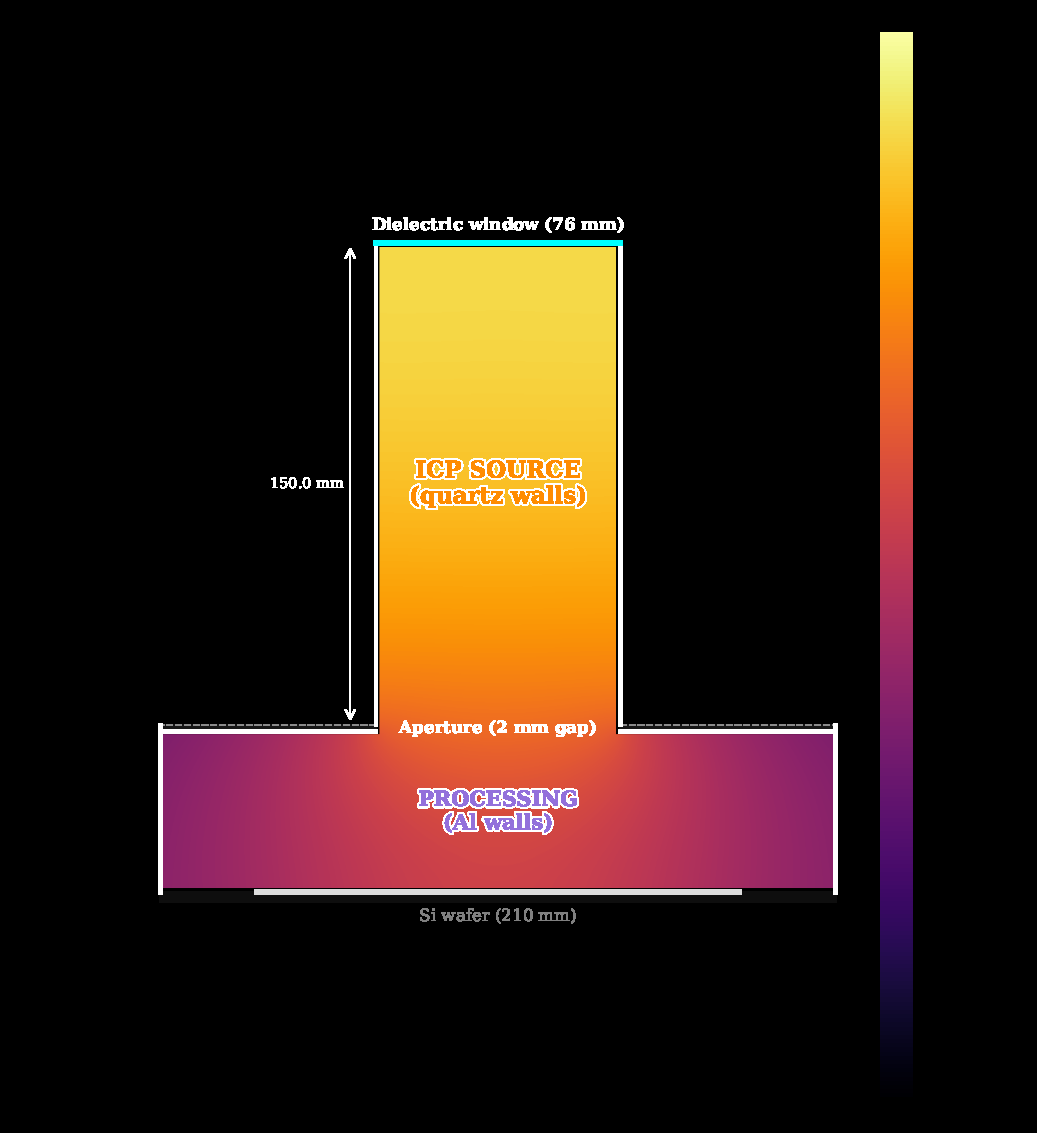
\includegraphics[width=0.55\textwidth,height=0.82\textheight,keepaspectratio]{fig_cross_section_F}
\end{frame}

% ──────────────────────────────────────────
\begin{frame}{Results: Wafer-Level Radial Profiles}
  \centering
  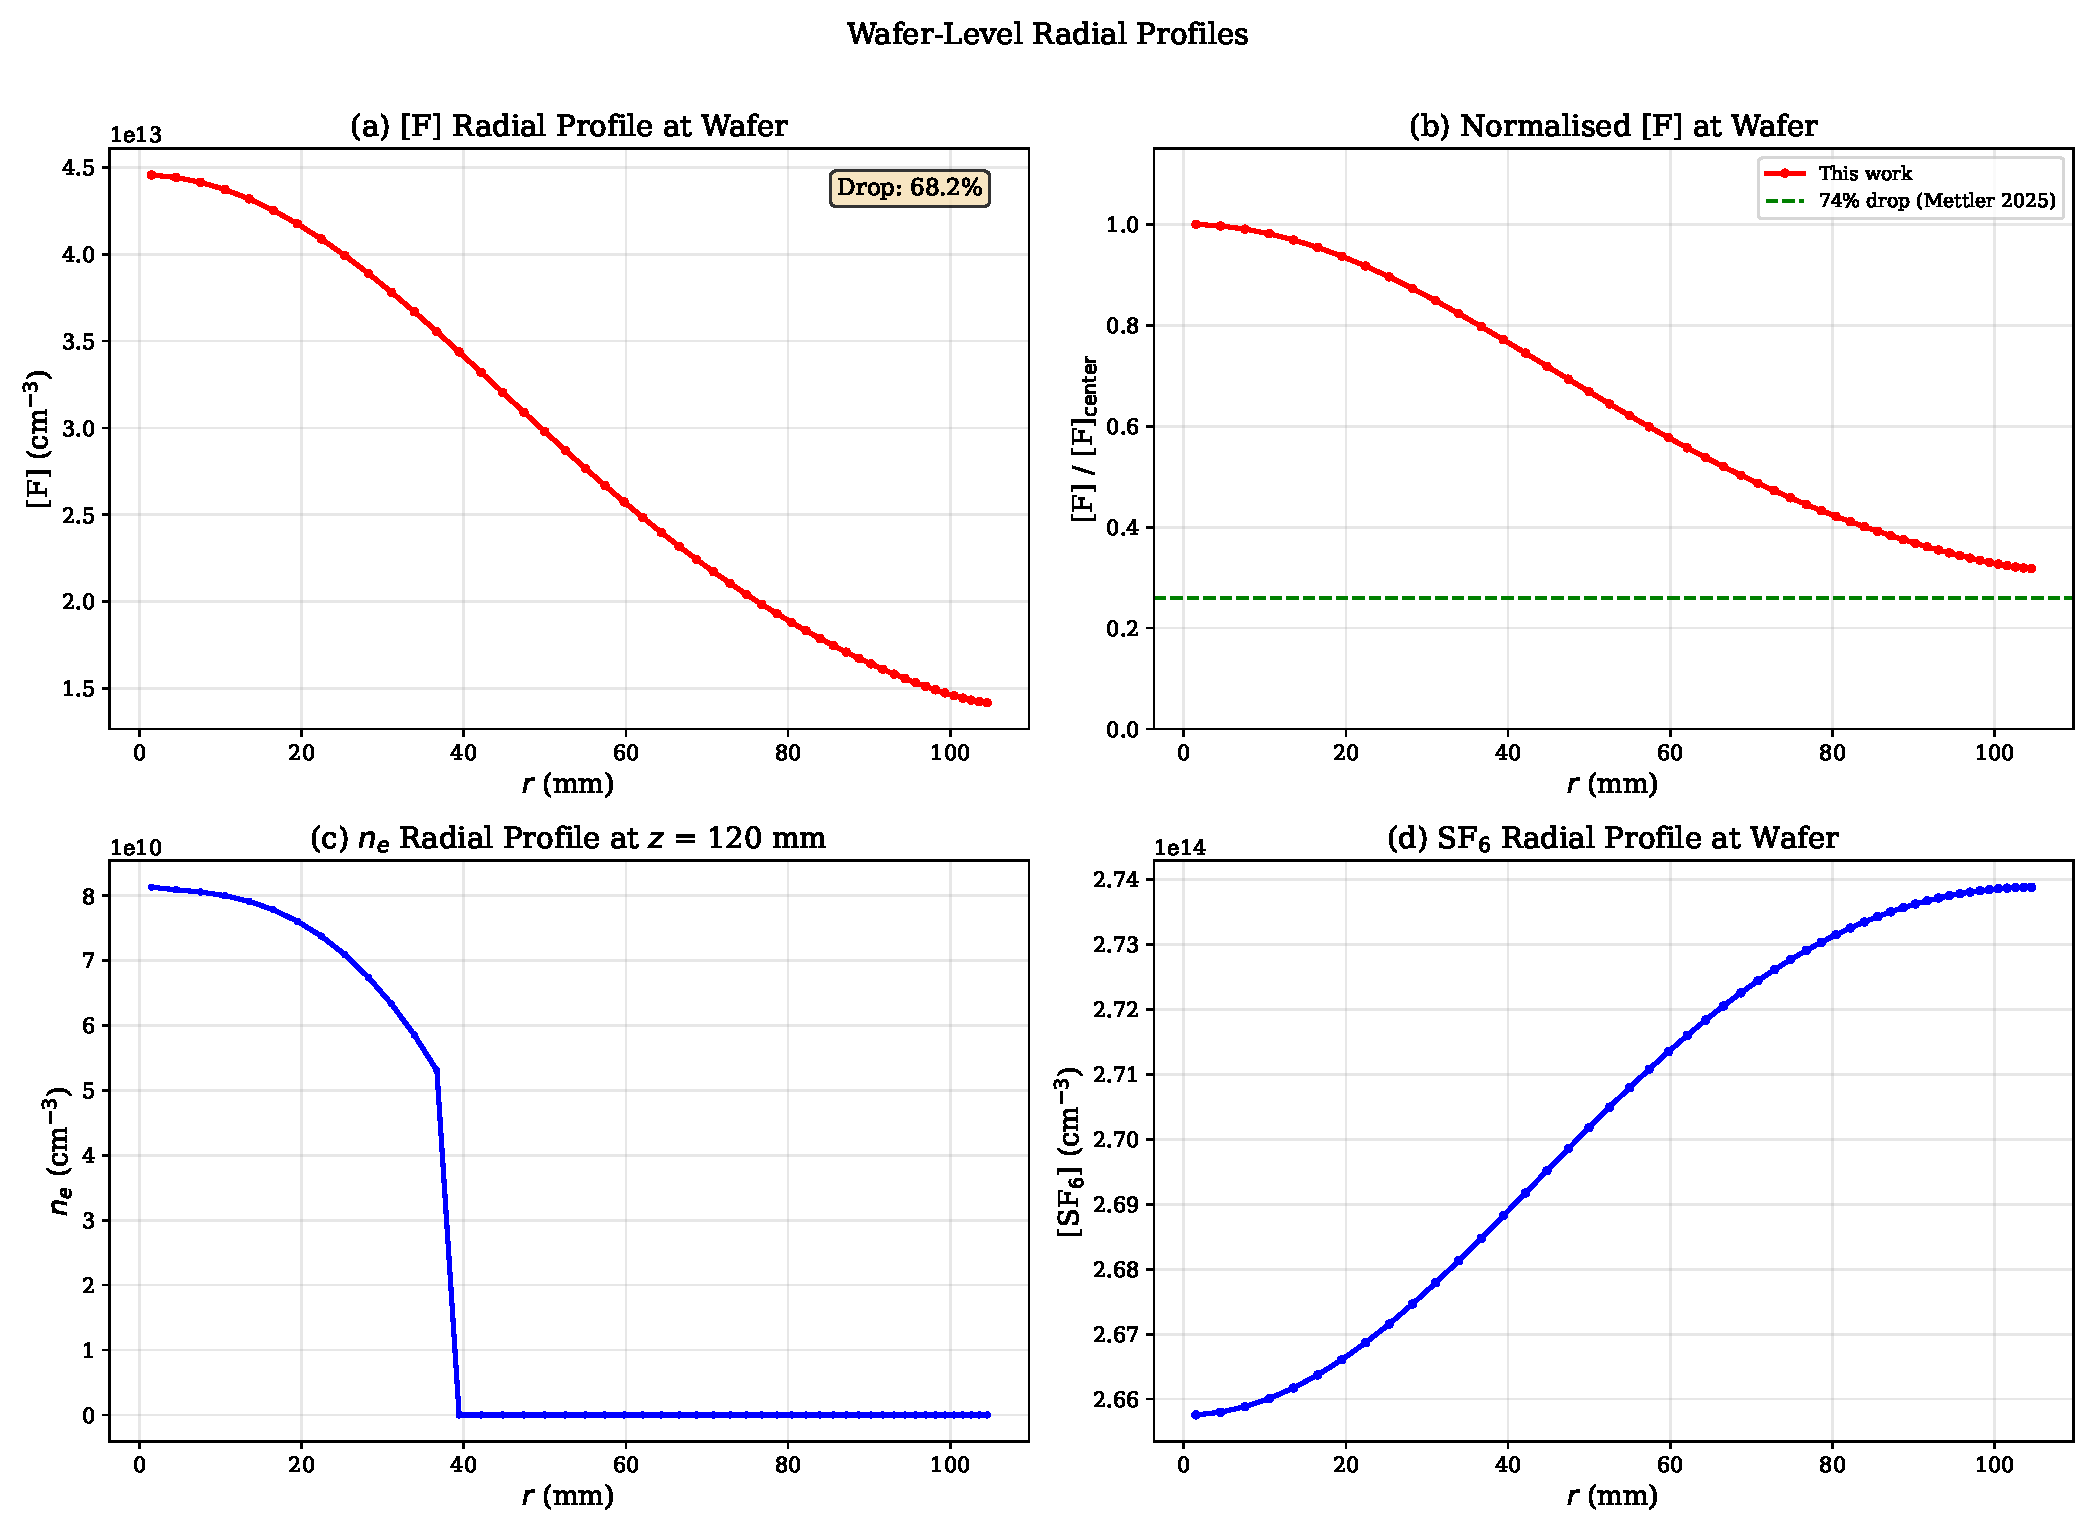
\includegraphics[width=0.95\textwidth,height=0.78\textheight,keepaspectratio]{fig_wafer_profiles}
\end{frame}

% ──────────────────────────────────────────
\begin{frame}{Results: Summary}
  \centering
  \footnotesize
  \begin{tabular}{@{}lccc@{}}
    \toprule
    \textbf{Quantity} & \textbf{Phase 1} & \textbf{Stage 10} & \textbf{Mettler Expt} \\
    \midrule
    {[F] drop}         & \textbf{77.8\%}  & 74\%              & 74\% \\
    $\eta$             & 0.430            & 0.43 (prescribed) & --- \\
    $n_{e,\text{avg}}$ & $3.0\times10^{16}$ m$^{-3}$ & --- & --- \\
    $\Te$ avg          & \SI{3.8}{\eV}    & \SI{2.3}{\eV}     & --- \\
    $|E_{\theta,\text{rms}}|_\text{max}$ & \SI{456}{\volt/\meter} & --- & --- \\
    Picard iterations  & 20               & N/A               & --- \\
    Total time         & \SI{112}{\second} & \SI{12}{\second}  & --- \\
    \bottomrule
  \end{tabular}

  \vspace{0.4cm}
  \normalsize
  \textbf{77.8\% [F] drop from first-principles physics with zero calibration}\\
  (within 4 pp of experimental 74\%)
\end{frame}

% ──────────────────────────────────────────
\begin{frame}{Discussion: 77.8\% vs.\ 74\%}
  \begin{itemize}[]
    \item The 3.8 pp gap reflects the physics difference between:
    \begin{itemize}[]
      \item \textbf{Phase 1}: self-consistent $n_e$ from FDTD power profile (peaks at $r\approx$ 20 mm)
      \item \textbf{Stage 10}: prescribed Bessel-cosine $n_e$ (peaks at $r = 0$)
    \end{itemize}
    \item More on-axis $n_e$ $\Rightarrow$ more central F production $\Rightarrow$ slightly larger drop
    \item \textbf{Three physics improvements} to close the gap naturally:
    \begin{enumerate}[]
      \item Electron energy transport PDE (smooths $\Te$ toward axis)
      \item Self-consistent FDTD (re-run with updated $\sigma$)
      \item EN-corrected h-factors for wall loss
    \end{enumerate}
    \item None require calibration --- they are physics additions for Phase 2
    \item $\gamma_\text{Al} = 0.18$ sensitivity: $\pm$10\% gives $\pm$5 pp in [F] drop
  \end{itemize}
\end{frame}


% ══════════════════════════════════════════════════════════════
\section{Part IV: Future Work}
% ══════════════════════════════════════════════════════════════

% ──────────────────────────────────────────
\begin{frame}{Roadmap: Phases 2--4}
  \textbf{Phase 2: Electron Kinetics}
  \begin{itemize}[]
    \item Tier 1: BOLSIG+ offline lookup tables for non-Maxwellian EEDF
    \item Tier 2: PINN Boltzmann solver for ML-accelerated rates
    \item Tier 3: PIC-MCC for one-time gold-standard validation
    \item EMCS (Electron Monte Carlo) as intermediate approach
  \end{itemize}
  \vspace{0.3cm}
  \textbf{Phase 3: ML-DTPM Surrogate}
  \begin{itemize}[]
    \item MLP / DeepONet / Autoencoder for real-time prediction
    \item Training: 5000+ parameter-sweep runs $\Rightarrow$ $(P, p, x_\mathrm{Ar}) \to$ [F] profile
  \end{itemize}
  \vspace{0.3cm}
  \textbf{Phase 4: Module Migration (M09--M18)}
  \begin{itemize}[]
    \item Ion transport, sheath model, surface chemistry, etch profile prediction
  \end{itemize}
\end{frame}

% ──────────────────────────────────────────
\begin{frame}{Summary}
  \begin{enumerate}
    \item \textbf{EM pipeline} (M01--M08): modular, validated, from RF circuit to EEDF
    \item \textbf{SF$_6$ chemistry}: 54-reaction mechanism + material-specific wall chemistry on TEL geometry $\Rightarrow$ 74\% [F] drop (Stage 10)
    \item \textbf{Phase 1 integration}: cylindrical FDTD + Picard coupling replaces prescribed $\eta$, $n_e$, $\Te$ with self-consistent physics
    \item \textbf{Result}: \textbf{77.8\% [F] drop} from first principles (4 pp from experiment)
    \item \textbf{Performance}: \SI{112}{\second} total (\SI{30}{\second} FDTD + \SI{82}{\second} chemistry)
    \item \textbf{Next}: electron kinetics (Phase 2), ML surrogate (Phase 3)
  \end{enumerate}

  \vspace{0.4cm}
  \centering
  \large\textbf{Code: \texttt{5.Phase1\_EM\_Chemistry\_Merged/}}
\end{frame}

% ══════════════════════════════════════════
\begin{frame}{References}
  \scriptsize
  \begin{enumerate}[]
    \item Lieberman \& Lichtenberg, \textit{Principles of Plasma Discharges}, 2nd ed. (2005)
    \item Kokkoris et al., \textit{J. Phys. D} \textbf{42}, 055209 (2009)
    \item Lallement et al., \textit{Plasma Sources Sci. Technol.} \textbf{18}, 025001 (2009)
    \item Mettler, PhD Dissertation, UIUC (2025)
    \item Yee, \textit{IEEE Trans. Antennas Propag.} \textbf{14}, 302 (1966)
    \item Mur, \textit{IEEE Trans. EMC} \textbf{23}, 377 (1981)
    \item Boris, \textit{Proc.\ 4th Conf.\ Num.\ Sim.\ Plasmas} (1970)
    \item Birdsall \& Langdon, \textit{Plasma Physics via Computer Simulation} (1991)
    \item Ryan \& Plumb, \textit{Plasma Chem. Plasma Process.} \textbf{10}, 207 (1990)
    \item Lee \& Lieberman, \textit{J. Vac. Sci. Technol. A} \textbf{13}, 368 (1995)
    \item Kim et al., \textit{Sci. Rep.} \textbf{13}, 16564 (2023) --- PINN Boltzmann
    \item Hagelaar \& Pitchford, \textit{Plasma Sources Sci. Technol.} \textbf{14}, 722 (2005)
  \end{enumerate}
\end{frame}

\end{document}
